

Objekto pozicijos nustatymas, naudojant pagreičio jutiklius, remiasi prielaida, jog objektas lieka ramybės būsenoje tol, kol jį nepradeda veikti kažkokia išorinė jėga. 
Tokia jėga suteikia objektui pagreitį. 
Jeigu rastą pagreitį galima išmatuoti ir suintegruoti, pagreičio ir pozicijos kitimas gali būti išmatuotas. 
Reikia nepamiršti, kad tokiu atveju matavimą sudarys dvi komponentės -- gravitacijos pagreitis ir išorinės veikiančios jėgos pagreitis. 
Norint pašalinti gravitacijos komponentę iš pagreičio matavimo, reikia nustatyti, kokiu kampu pagreičio jutiklis yra vertikalės atžvilgiu.
Kampui matuoti reikalingas kitas jutiklis - giroskopas.
Jis matuoja kampo pokyčio greitį, kurį matematiškai integruojant, galima rasti kampo greičio pokytį \cite{sukkarieh2000low}.

Akcelerometru nustatomas stebimo objekto pagreičio matavimo įvertis.
Dažniausiai tokie matavimai yra žymimi $x$ (judėjimas tiesiai), $y$ (šonu) ir $z$ (vertikaliai). 
Giroskopas suteikia matavimus, kurie dengia nurodytas ašis ir yra užrašomi $\theta$, sūkiui, $\beta$ polinkiui ir $\gamma$ vingiavimui, kaip pavaizduota \ref{tikz:axis_of_the_system} pav. 
Tokių inercinių įverčių naudojimas turi pagrindinį privalumą -- stebimo objekto polinkis ir pagreitis gali būti vertinami bet kokioje navigacijoje.  

\begin{figure}[b]
    \centering
    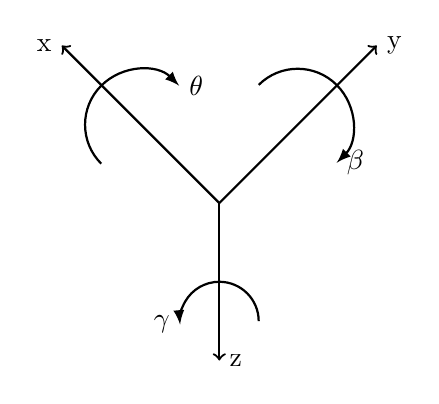
\begin{tikzpicture}
        % axis
        \draw[thick, black, ->] (0,0) -- ( 2, 2) node [right] {y};
        \draw[thick, black, ->] (0,0) -- (-2, 2) node [left] {x}; 
        \draw[thick, black, ->] (0,0) -- ( 0,-2) node [right] {z};
        % arc
        \draw[thick, -latex] ( 0.5,  1.5) arc (135:-45:0.70) node [right] {$\beta$}; 
        \draw[thick, -latex] (-1.5,  0.5) arc (225:45:0.70) node [right] {$\theta$};
        \draw[thick, -latex] ( 0.5, -1.5) arc (0:185:0.5) node [left] {$\gamma$};
    \end{tikzpicture}
    \caption{Objekto pozicijos pagreičio pokyčio ašys, $x$, $y$ ir $z$. Sūkio matmenys apie ašis $\theta$, $\beta$ ir $\gamma$}
    \label{tikz:axis_of_the_system}
\end{figure}

\textbf{Darbo aktualumas}

Pagreičio navigacijos sistemos yra labai plačiai naudojamos lėktuvuose, raketose, kosmoso laivuose, povandeniniuose ir vandens laivuose \cite{woodman2007introduction}.
Progresas, gaminant MEMS įrenginius, sudarė galimybes kurti mažas ir lengvas navigacines sistemas.
Tokie privalumai leidžia įrenginius naudoti ir kitose srityse, pavyzdžiui matuojant kaip žmogaus ir gyvūnų judesius \cite{schlomer2008gesture,suvorova2012action}.

\textbf{Darbo problema}

Vis dėlto reikia nepamiršti ir apie klaidas, kurias sukelia nuolatinė dedamoji, santykio įverčiai ir nelinijinės sistemos įtaka jutiklio verčių nuskaitymo metu.
Tokios klaidos yra pagrindinė priežastis navigacinėje sistemoje neapibrėžtumams per laiko vienetą atsirasti. 
Neapibrėžtumas sąlygoja akselerometro įverčius, kuriuos labai sunku atskirti nuo gravitacinio lauko ir objekto judėjimo, todėl objekto pozicijos matavimas toliau yra dar netikslesnis. 
Kadangi inerciniai jutikliai yra tokio tipo, kuriems yra labai svarbi tiksli prieš tai buvusi pozicija, bet kokia klaida skaičiuojant prieš tai buvusia pozicija, įtakoja ir dabartinės pozicijos skaičiavimą. 
Tokiu būdu, su laiku navigacinė sistema tampa visiškai neapibrėžta ir praranda visą savo vertę.

\textbf{Darbo tikslas}

Darbo metu bus įgyvendinta padėties nustatymo sistema, taikant MEMS tipo jutiklius ir mikrovaldiklį.
Pasirinktas jutiklis yra \textit{MPU-9250} \cite{MPU-96:online}, devynių ašių judesio sekimo įrenginys, kuris yra pritaikomas mobiliems telefonams, nešiojamiems jutikliams ir kitoms reikmėms.
Naudojama \textit{STM32 Nucleo} plokštė yra įperkamas ir lankstus būdas naudotojams išbandyti idėjas ir sukurti prototipą su bet kuriuo iš STM32 serijos mikro-valdikliu \cite{STM3258:online}.

\textbf{Darbo uždaviniai}

Pirmas darbo uždavinys yra aptarti MEMS tipo pagreičio ir giroskopo jutiklius.
Patarti nuolatinių dedamųjų, kalibravimo ir klaidų atsiradimo klausimus.
Antras uždavinys yra atlikti esamų sistemų analizę.
Trečias uždavinys yra aptarti aparatinę įrangą, kuri bus panaudoja sprendimui įgyvendinti.
Ketvirtas uždavinys yra atlikti galimų sistemų tyrimą ir pasirinkti labiausiai tinkamą sprendimą.
Paskutinis uždavinys yra įgyvendinti pasirinktą sistemą įterptinėje sistemoje.